% Gemini theme
% https://github.com/anishathalye/gemini

\documentclass[final,16pt]{beamer}

% ====================
% Packages
% ====================

\usepackage[T1]{fontenc}
\usepackage{lmodern}
\usepackage[size=custom,width=120,height=91,scale=1.1]{beamerposter}
%\usepackage[size=custom,width=48in,height=36in,scale=1.1]{beamerposter}
%\setlength{\paperwidth}{48in} % A0 width: 46.8in
%\setlength{\paperheight}{36in} % A0 height: 33.1in
\usetheme{gemini}
\usecolortheme{gemini}
\usepackage{graphicx}
\usepackage{booktabs}
\usepackage{wrapfig}
\usepackage{tikz}
\usepackage{pgfplots}
\pgfplotsset{compat=1.14}

% ====================
% Lengths
% ====================

% If you have N columns, choose \sepwidth and \colwidth such that
% (N+1)*\sepwidth + N*\colwidth = \paperwidth
\newlength{\sepwidth}
\newlength{\colwidth}
\setlength{\sepwidth}{0.025\paperwidth}
\setlength{\colwidth}{0.3\paperwidth}

\newcommand{\separatorcolumn}{\begin{column}{\sepwidth}\end{column}}

% ====================
% Title
% ====================

\title{A Deep Learning Approach for Detection, Semantic Segmentation \\
and Density Classification of Smoke in Satellite Imagery}

\author{Rey Koki \inst{1, 2, 3} \and Michael McCabe \inst{1} \and Jebb Stewart \inst{2} \and Christina Kumler \inst{2,3} \and Jed Brown \inst{1} \and Wilfrid Schroeder \inst{4}}

\institute[shortinst] {\inst{1} Computer Science Department, CU Boulder, Boulder, CO  \samelineand \inst{2} NOAA's Global Systems Laboratory, Boulder, CO \samelineand \inst{3} Cooperative Institute for Research in Environmental Sciences, CU Boulder, Boulder, CO \samelineand \inst{4} NOAA NESDIS, College Park, MD}

% ====================
% Footer (optional)
% ====================

\footercontent{
  Presentation ID\# 1131851\hfill
  %CIRES Innovative Research Program Poster Session\hfill
  American Geological Union Fall 2022, Chicago, IL\hfill
  \href{mailto:rey.koki@colorado.edu}{rey.koki@colorado.edu}}
% (can be left out to remove footer)

% ====================
% Logo (optional)
% ====================

% use this to include logos on the left and/or right side of the header:
% \logoright{\includegraphics[height=7cm]{logo1.pdf}}
% \logoleft{\includegraphics[height=7cm]{logo2.pdf}}

% ====================
% Body
% ====================

\begin{document}

\addtobeamertemplate{headline}{}
{
\begin{tikzpicture}[remember picture,overlay]
\node [shift={(-10 cm,-8cm)}] at (current page.north east) {
\includegraphics[height=2.7cm]{figures/logo.png}};
\end{tikzpicture}
\begin{tikzpicture}[remember picture,overlay]
\node [shift={(-12 cm,-4cm)}] at (current page.north east) {
\includegraphics[height=3.5cm]{figures/cireslogo.png}};
\end{tikzpicture}
\begin{tikzpicture}[remember picture,overlay]
\node [shift={(-4 cm,-4cm)}] at (current page.north east) {
\includegraphics[height=4.5cm]{figures/noaa.png}};
\end{tikzpicture}
}

\begin{frame}[t]
\begin{columns}[t]
\separatorcolumn

\begin{column}{\colwidth}

  \begin{exampleblock}{Contributions}
    \begin{enumerate}
      \item{Created database of labeled satellite imagery using smoke annotations}
      \item{Built deep learning arch to perform detection, classification and segmentation}
      \item{Introduced thermometer encoding for ordinal ranking of smoke density}
      \item{Calculated metrics and analyzed performance}
    \end{enumerate}

  \end{exampleblock}

  \begin{block}{Motivation}

   Because of NOAA's large quantity of historical, analyst-labeled data, we can deploy deep learning methods that leverage big data in order to create an automated algorithm for localizing smoke in satellite imagery. Our goal is to create a human in the loop algorithm that will lower the required labor.

  \end{block}

  \begin{block}{Smoke Labels}

    \begin{wrapfigure}{r}{0.75\textwidth}
      \centering
      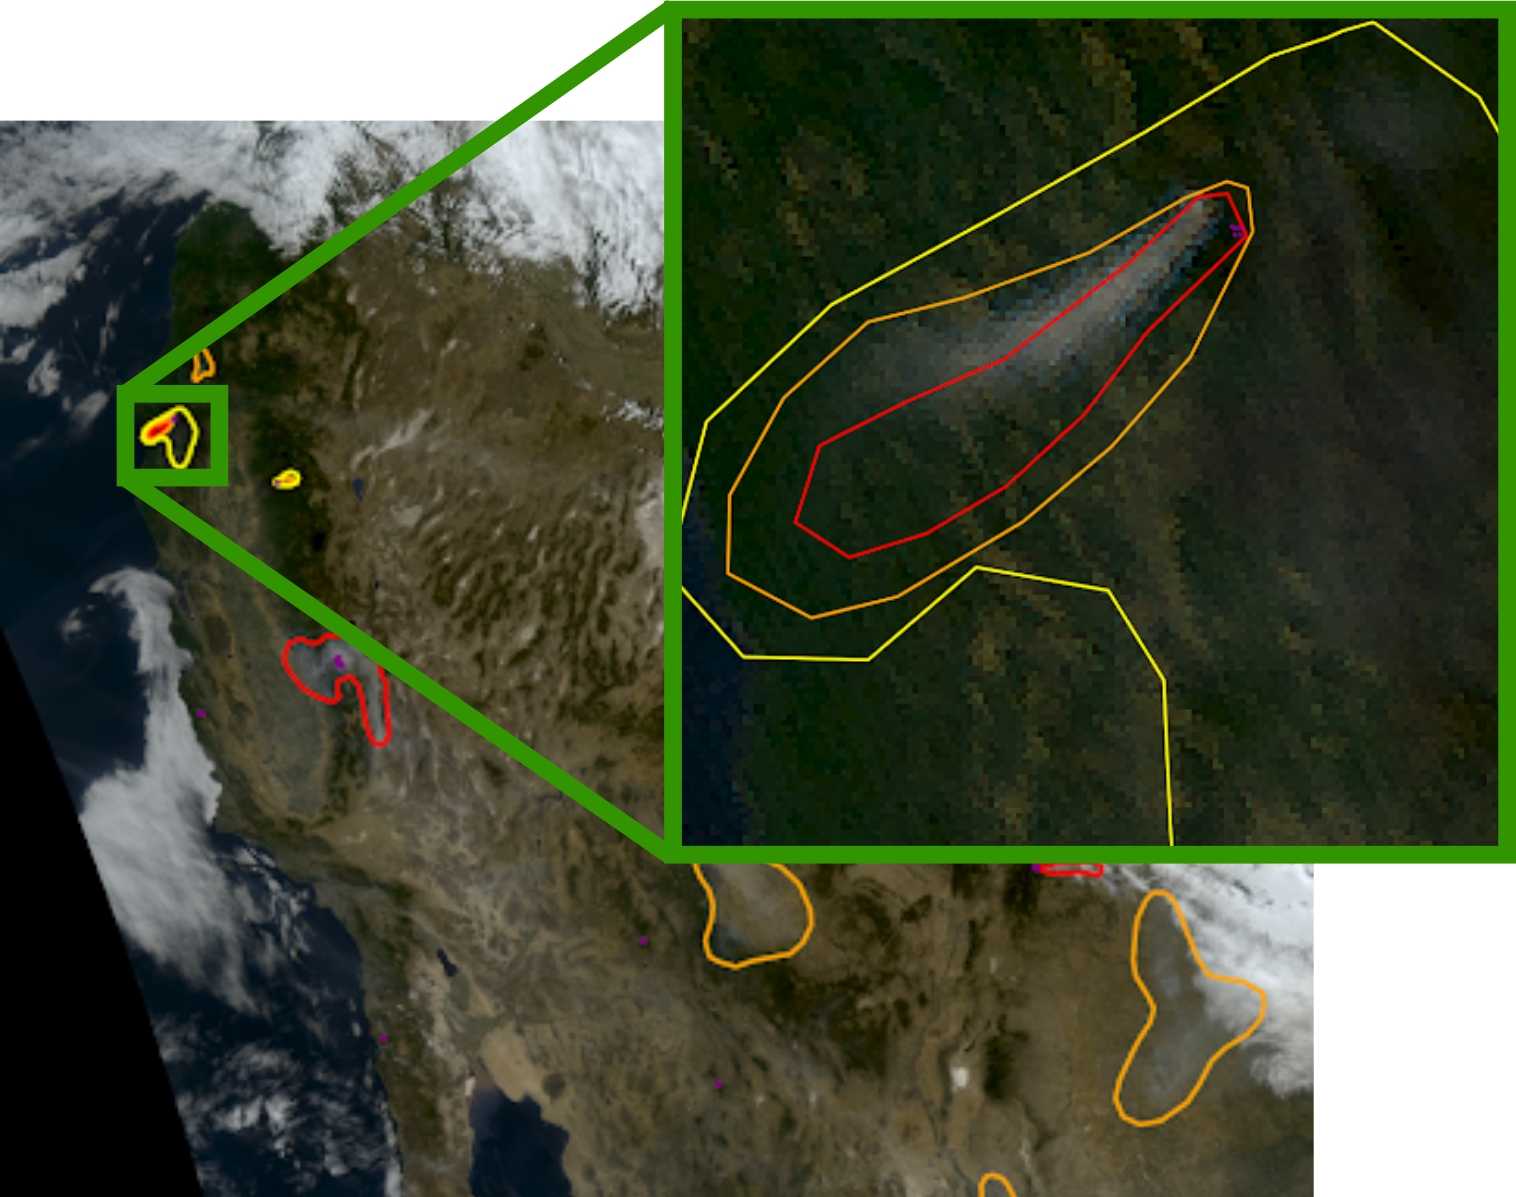
\includegraphics[width=0.7\textwidth]{figures/zoomed.png}
      \caption{GOES-EAST imagery with corresponding HMS smoke annotations. The color of the outlines correspond to the density.}
    \end{wrapfigure}
    The Hazard Mapping Systems (HMS) team is continuously providing fire and smoke products for North America. Smoke plumes are identified, outlined and classified by by their particulate density as either heavy, medium or low (figure 1). The HMS smoke labels are created using a timeseries of imagery that can span up to 5 hours, complicating the data if there are shifts in smoke position.
  \end{block}


  \begin{block}{Satellite Imagery}
    NOAA’s GOES satellites provide uninterrupted imagery that we use as input to our model. Leveraging the physics of the problem, we apply feature engineering in order for our model to better interpret our data.
    \begin{figure}
      \centering
      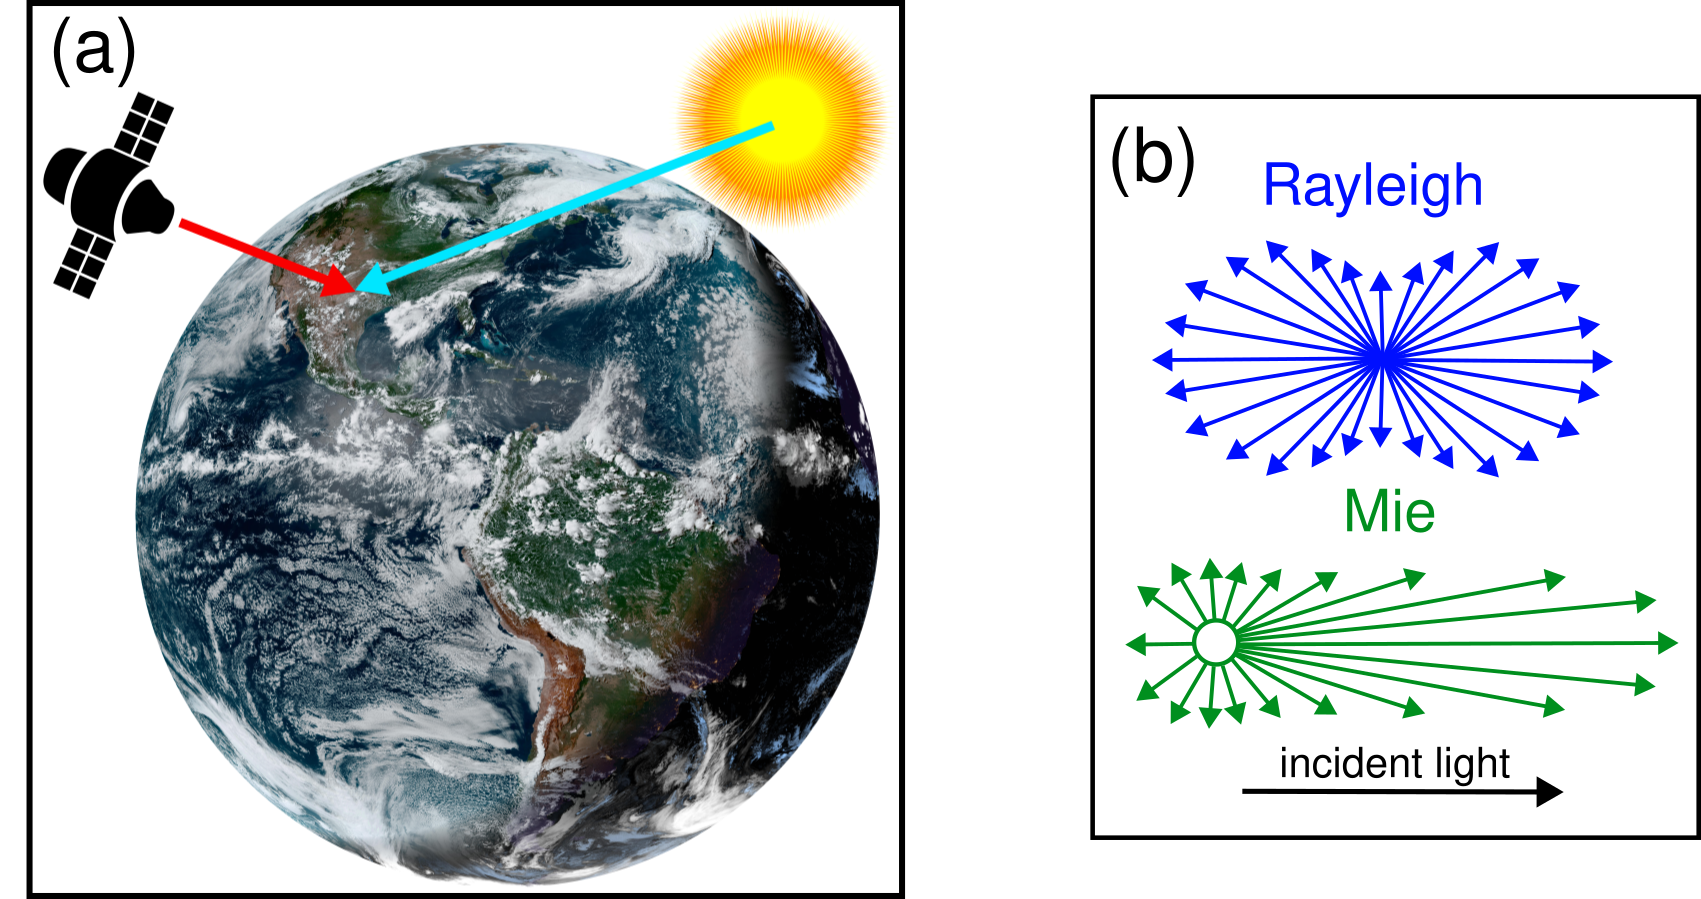
\includegraphics[width=33cm]{figures/LOS_scattering.png}
      \caption{(a) GOES imagery with line of sight illustrated for the sun and satellite. (b) Illustration of how Mie scattering favors forward rather than backward scattering.}
    \end{figure}

  \end{block}

\end{column}

\separatorcolumn

\begin{column}{\colwidth}

  \begin{block}{Semantic Segmentation}
    We use semantic segmenation (figure 3) to classify the smoke on a pixel by pixle basis.
    \begin{figure}
      \centering
      \includegraphics[width=20cm]{figures/semantic_seg.png}
      \caption{Comparison to traditional image or object classication.}
    \end{figure}
  \end{block}

  \begin{block}{Dataset and Workflow}
    Training set included 63,076 samples from 2019, 2000 and 2022 data. Validation set contain 8,227 samples from odd weeks in 2021, test set contains 7,729 samples from even weeks in 2021. All data is within the continental United States.
    \begin{figure}
      \centering
      \includegraphics[width=37cm]{figures/workflow.png}
      \caption{Workflow from feature engineering to the output of the model. The deep learning architecture consists of ResNeXt \cite{resnext} that extracts features from the data and DeepLabV3+ \cite{deeplab} that performs semantic segmentation.}
    \end{figure}
  \end{block}

  \vspace{-1cm}
  \begin{block}{Thermometer Encoding}

    \begin{table}
      \centering
      \begin{tabular}{| p{8cm} | p{5cm} |}
        \hline
        \vspace{.005cm}\textbf{no smoke} & \vspace{.005cm}\hspace{.9cm}[0, 0, 0] \\
        \hline
        \vspace{.005cm}\textbf{low smoke} & \vspace{.005cm}\hspace{.9cm}[0, 0, 1] \\
        \hline
        \vspace{.005cm}\textbf{medium smoke} & \vspace{.005cm}\hspace{.9cm}[0, 1, 1] \\
        \hline
        \vspace{.005cm}\textbf{heavy smoke} & \vspace{.005cm}\hspace{.9cm}[1, 1, 1] \\
        \hline
      \end{tabular}
      \caption{We apply ordinal rankings so that the penalization is representative of density proximity.}
    \end{table}
  \end{block}


  \begin{block}{Discusion and Future Work}
    By taking advantage of physics based feature engineering, domain knowledge based architecture design and thermometer encodings, we were able to show state-of-the-art performance. Future work includes feature attribution to identify additional bands and pretraining the neural network weights.


  \end{block}


\end{column}


\separatorcolumn


\begin{column}{\colwidth}

  \begin{block}{Intersection over Union}
    \begin{minipage}{.6\textwidth}
        \begin{figure}
            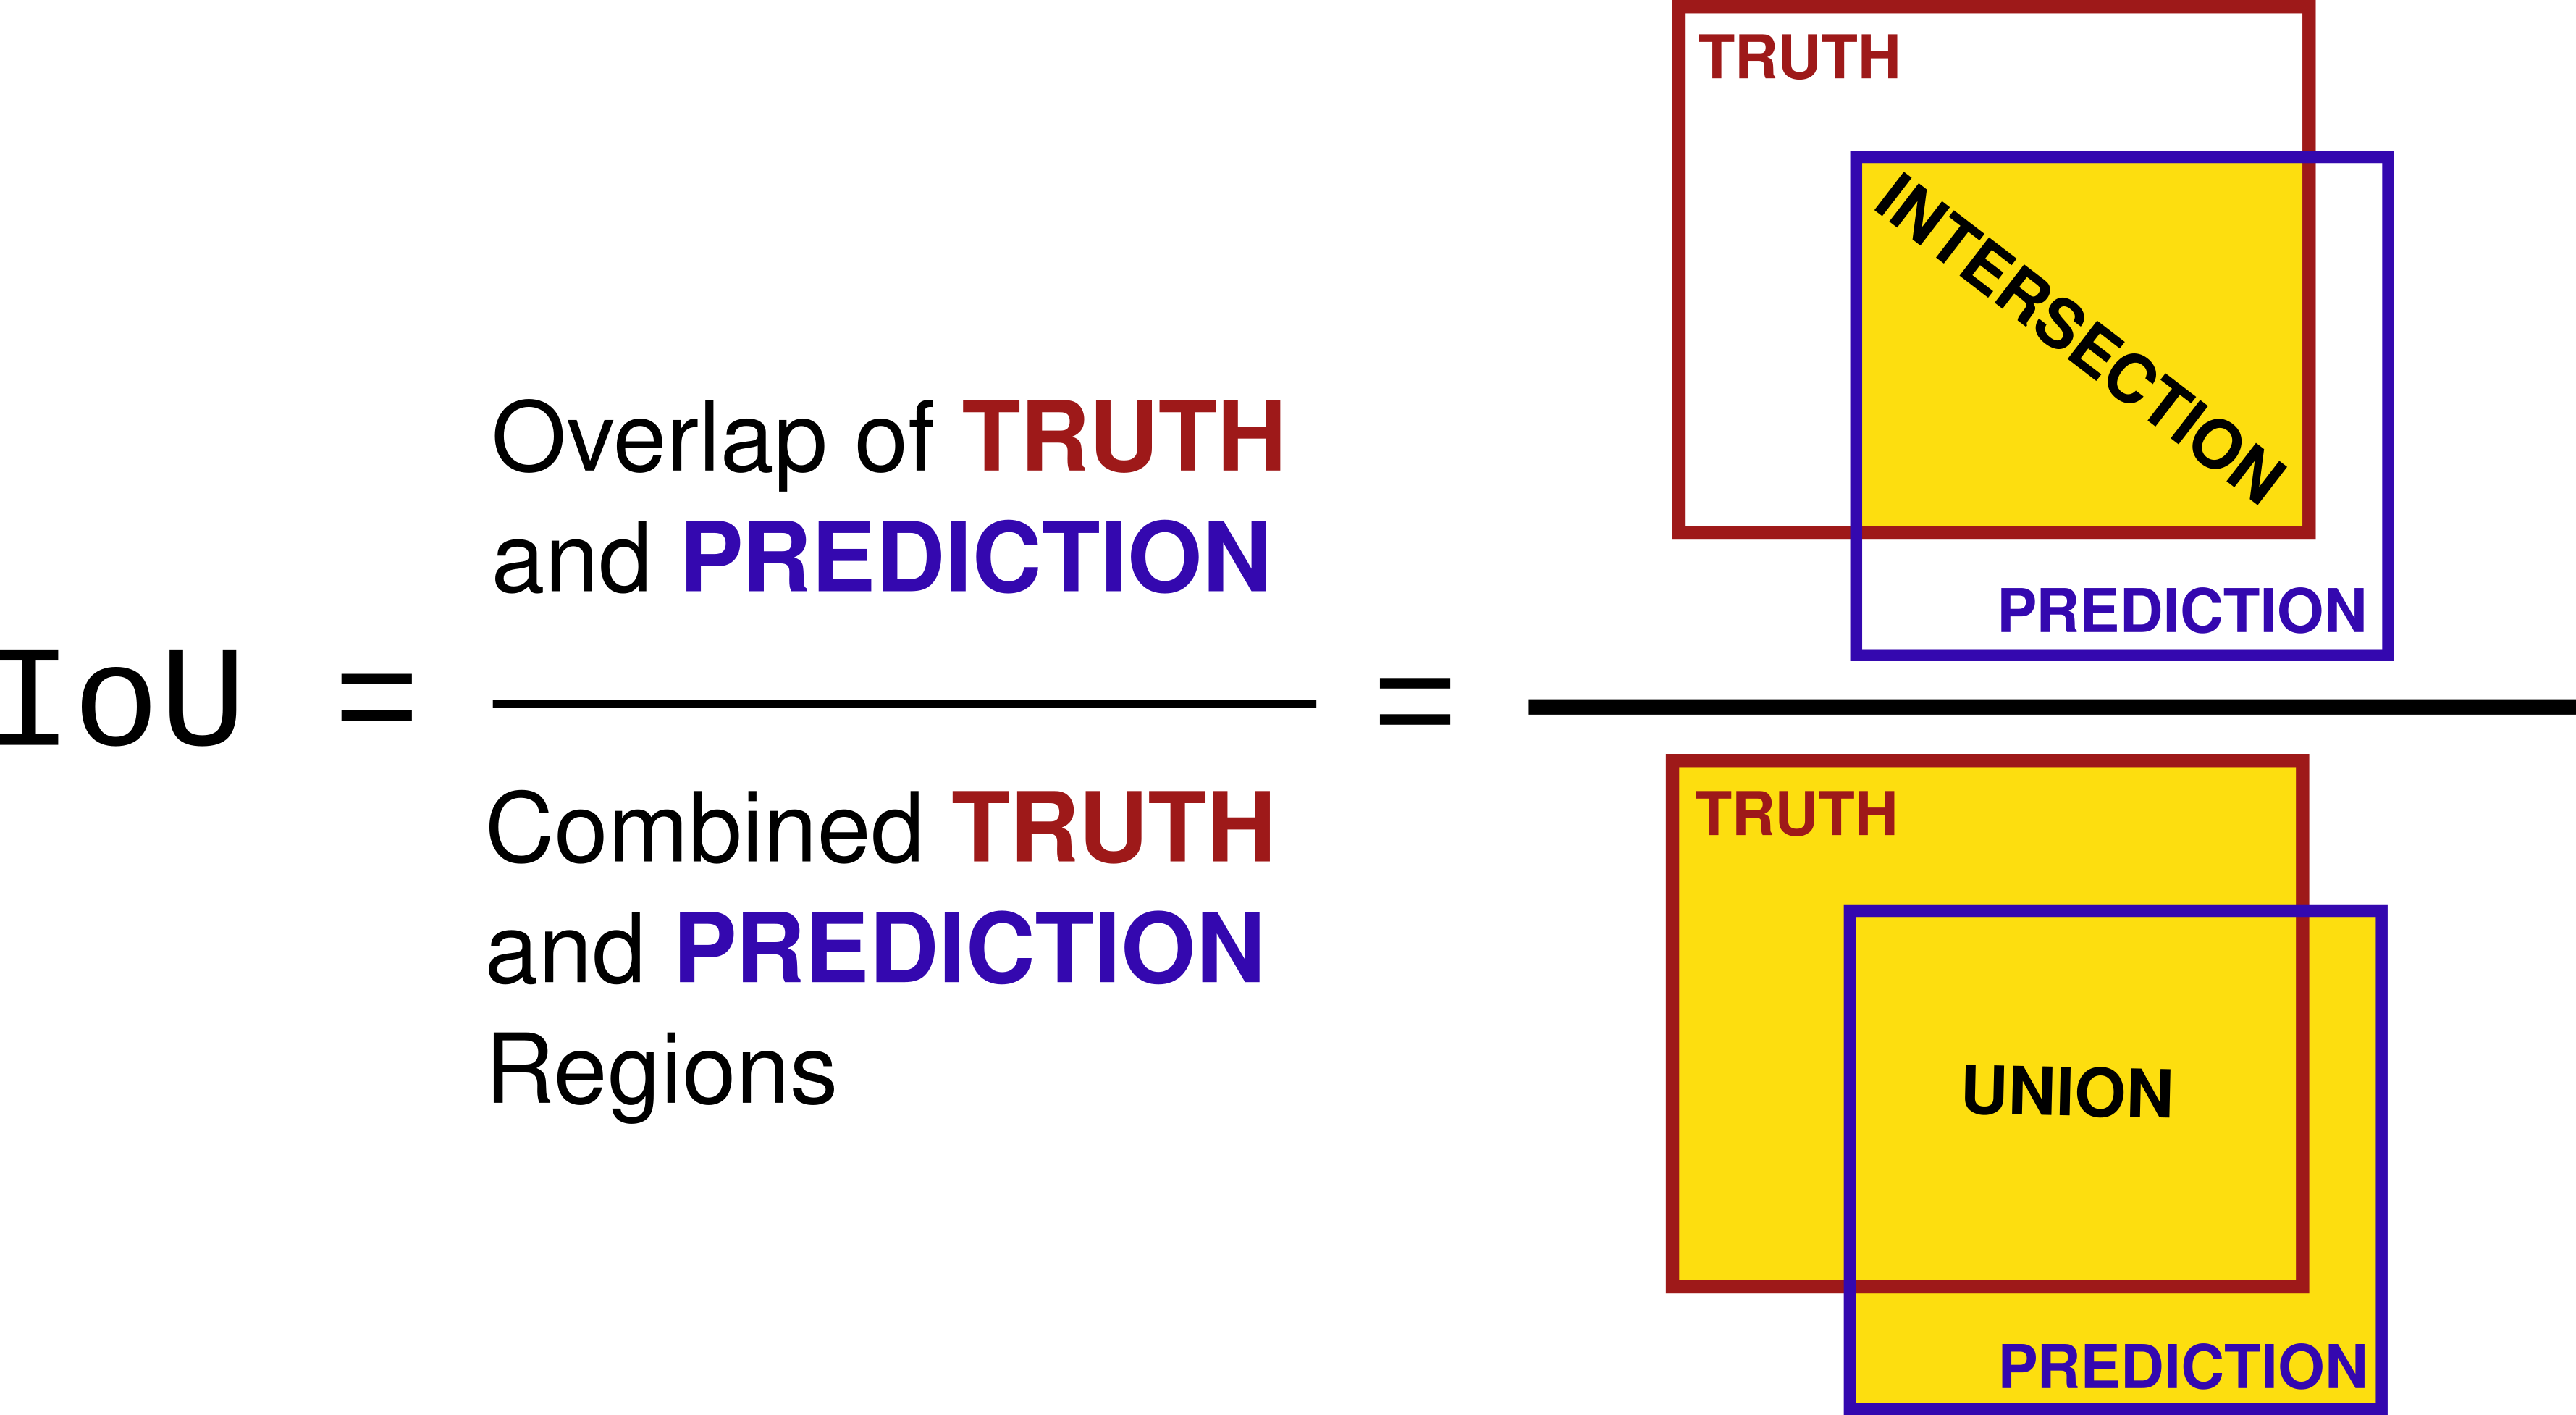
\includegraphics[width=.8\textwidth]{figures/IoU.png}
            \caption{To measure performance, we use the IoU metric.}
        \end{figure}
    \end{minipage}%
    \begin{minipage}{.4\textwidth}
        \begin{table}
          \centering
          \begin{tabular}{l c c }
            \toprule
            \textbf{density} & \textbf{IoU} & \textbf{CAIoU} \\
            \midrule
            low & 0.493 &  0.510 \\
            medium \,\,\, & \,\,\,0.540\,\,\, & \,\,\,0.781\,\,\\
            heavy & 0.440  & 0.752\\
            overall & 0.498 & 0.710\\
            \bottomrule
          \end{tabular}
          \caption{IoU and Class Averaged IoU results by density and over entire dataset.}
        \end{table}
    \end{minipage}
  \end{block}


  \vspace{-1cm}
  \begin{block}{Example Results}

        \begin{figure}
            \centering
            \includegraphics[width=.8\textwidth]{figures/truth_vs_pred_4_exs.png }
            \caption{Visualization of the results for 4 test samples, IoU is calculated over all densities.}
        \end{figure}
        \begin{figure}
            \centering
            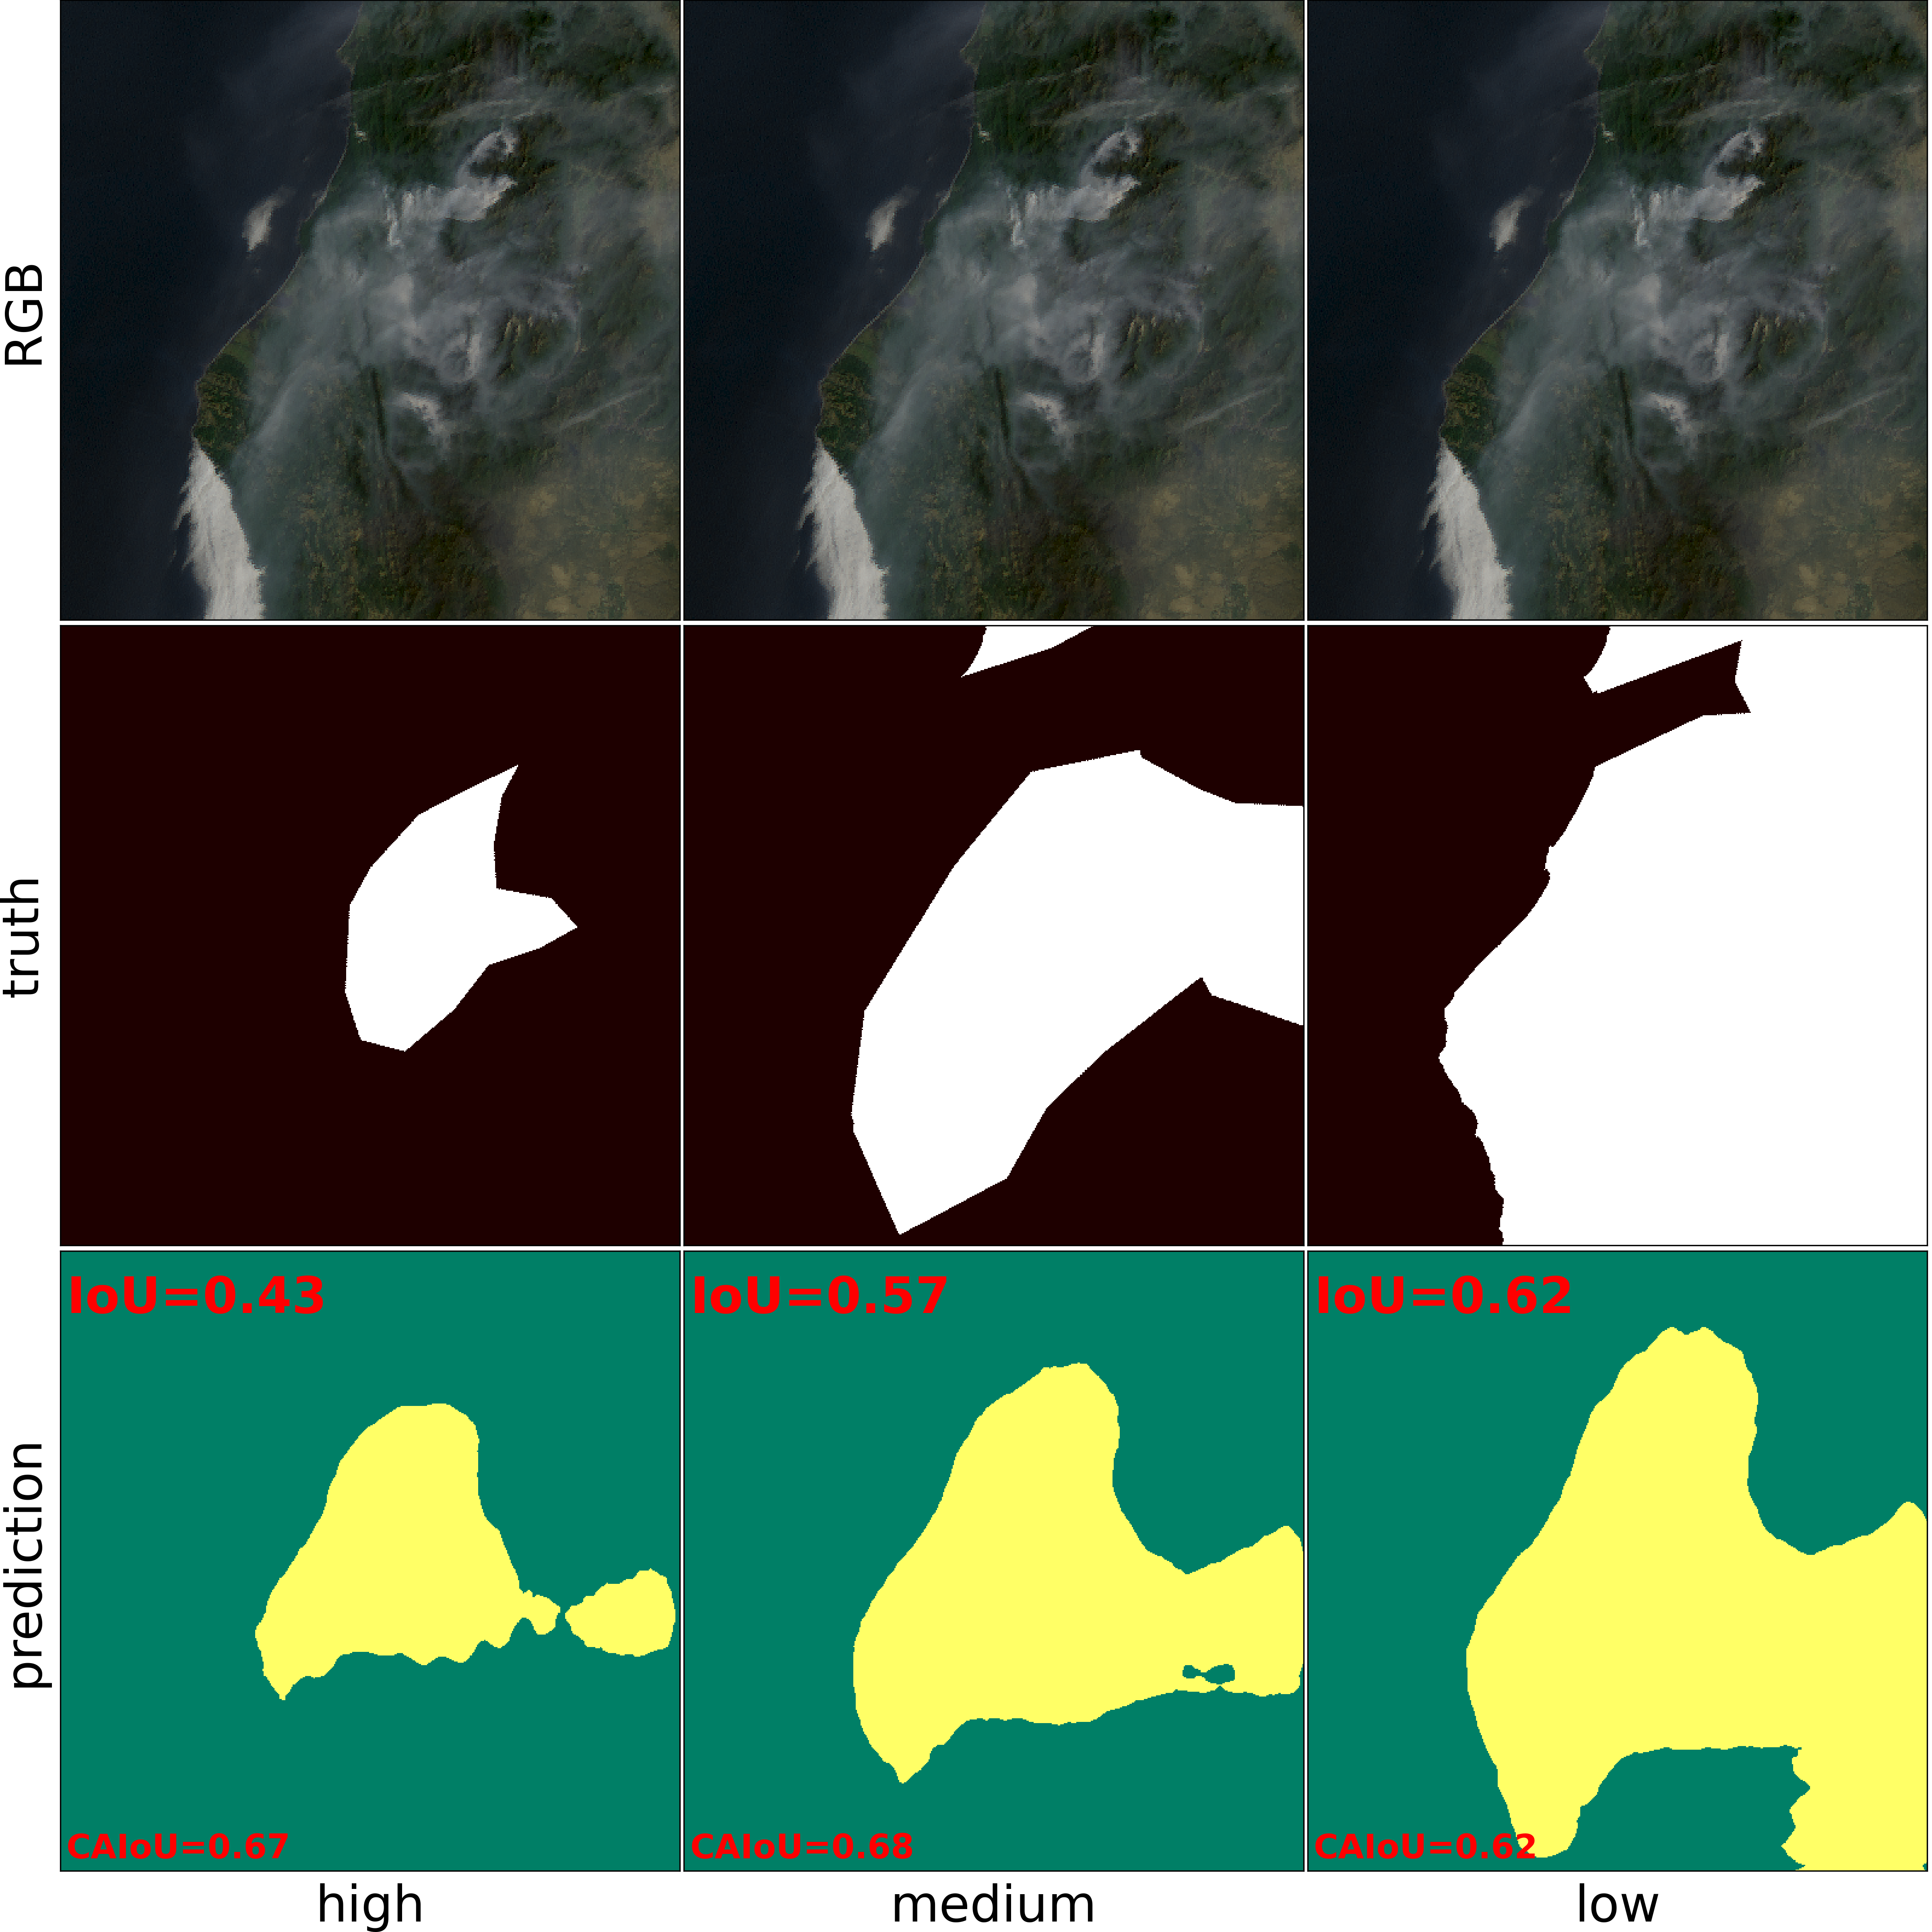
\includegraphics[width=.6\textwidth]{figures/vulture.png }
            \caption{Visualization of the results for 1 test sample, IoU is calculated per density.}
        \end{figure}
  \end{block}
  \vspace{-1cm}
  \begin{block}{References}
    \nocite{*}
    \footnotesize{\bibliographystyle{plain}\bibliography{poster}}
  \end{block}

\end{column}

\separatorcolumn
\end{columns}
\end{frame}

\end{document}
